\documentclass[pdftex,10pt,xcolor=svgnames]{beamer}

\mode<presentation>
{
  \usetheme{boxes}
  \usecolortheme[named=MidnightBlue]{structure}
  %\setbeamercolor{normal text}{bg=NavajoWhite!20}
  \usefonttheme{serif}
  \setbeamertemplate{navigation symbols}{}
  % Show frame number and author name in footline
  \setbeamertemplate{footline}[frame number]
  \addtobeamertemplate{footline}{\quad\textcolor{gray}{David Duvenaud and James Lloyd}}{}
  % Set frame titles in small capitals
  \setbeamerfont{frametitle}{shape=\scshape,family=\rmfamily}
  \setbeamercolor{frametitle}{bg=gray!60!white,fg=black}
  % Alerted text: blue (uncomment second line if theme sets alerted text to bold)
  \setbeamercolor{alerted text}{fg=blue}
  %\setbeamerfont*{alerted text}{}
  \setbeamertemplate{bibliography item}[text] %{\hbox{\donotcoloroutermaths$\blacktriangleright$}}
  \setbeamertemplate{bibliography entry title}{}
  \setbeamertemplate{bibliography entry author}{}
  \setbeamertemplate{bibliography entry note}{}
  \setbeamertemplate{bibliography entry location}{}

}
\usepackage[english]{babel}
\usepackage[latin1]{inputenc}
\usepackage{times}
\usepackage[T1]{fontenc}
\usepackage{hyperref}
\usepackage{multimedia}
\usepackage{eepic}
\usepackage{graphicx}
%\usepackage[nohug]{latexinclude/diagrams}
\usepackage{tikz}
\usetikzlibrary{calc}

%% \newcommand{\footlineextra}[1]{
%%     \begin{tikzpicture}[remember picture,overlay]
%%         \node[yshift=1.5ex,anchor=south east] at (current page.south east)
%% {#1};
%%     \end{tikzpicture}
%% }

\newcommand{\footlineextra}[1]{
    \begin{tikzpicture}[remember picture,overlay]
        \node[xshift=-5ex,yshift=-0.5ex,anchor=south east] at (current page.south east)
             {\mbox{\tiny \textcolor{MidnightBlue}{#1}}};
    \end{tikzpicture}
}

\def\sectionframe#1{
  {
    \setbeamertemplate{footline}{\empty}
    \begin{frame}{}
      \begin{center}
        \huge\sc #1
      \end{center}
    \end{frame}
  }
}



\usecolortheme{default}
% colours
\xdefinecolor{Black}{rgb}{0,0,0}
\xdefinecolor{White}{rgb}{1,1,1}
\xdefinecolor{DarkBlue}{rgb}{0,0,.7}
\xdefinecolor{DarkRed}{rgb}{.7,0,0}
\xdefinecolor{Red}{rgb}{.85,0,0}
\xdefinecolor{DarkGreen}{rgb}{0,.7,0}
\xdefinecolor{DarkMagenta}{rgb}{.6,0,.6}
\def\Black{\textcolor{Black}}
\def\White{\textcolor{White}}
\def\Blue{\textcolor{DarkBlue}}
\def\Magenta{\textcolor{DarkMagenta}}
\def\Red{\textcolor{Red}}
\def\Green{\textcolor{DarkGreen}}

\usepackage{alltt}
\usepackage{psfrag}
\usepackage{pstool}

\usepackage{picins}
\usepackage{tikz}
\usetikzlibrary{shapes.geometric,arrows,chains,matrix,positioning,scopes,calc}
\tikzstyle{mybox} = [draw=white, rectangle]

\title[] % (optional, use only with long paper titles)
{Introduction to probabilistic programming}

\author % (optional, use only with lots of authors)
{David Duvenaud and James Lloyd}
% - Use the \inst{?} command only if the authors have different
%   affiliation.

\institute[] % (optional, but mostly needed)
{University of Cambridge}
% - Use the \inst command only if there are several affiliations.
% - Keep it simple, no one is interested in your street address.

\date % (optional)
{\empty}

\subject{Talks}

\usetikzlibrary{shapes.geometric,arrows,chains,matrix,positioning,scopes}
 \makeatletter
 \tikzset{join/.code=\tikzset{after node path={%
       \ifx\tikzchainprevious\pgfutil@empty\else(\tikzchainprevious)%
       edge[every join]#1(\tikzchaincurrent)\fi}}
 }
 \tikzset{>=stealth',every on chain/.append style={join},
   every join/.style={->}
 }

\tikzstyle{mybox} = [draw=white, rectangle]
\usepackage{ifthen}
\usepackage{booktabs}

% Custom definitions
\def\simiid{\sim_{\mbox{\tiny iid}}}

%%%%%%%%%%%%%%%%%%%%%%%%%%%%%%%%%%%%%%%%%%%%%%%%%%%%%%%%%%
%%%% EDITING HELPER FUNCTIONS  %%%%%%%%%%%%%%%%%%%%%%%%%%%
%%%%%%%%%%%%%%%%%%%%%%%%%%%%%%%%%%%%%%%%%%%%%%%%%%%%%%%%%%

%% NA: needs attention (rough writing whose correctness needs to be verified)
%% TBD: instructions for how to fix a gap ("Describe the propagation by ...")
%% PROBLEM: bug or missing crucial bit 

%% use \fXXX versions of these macros to put additional explanation into a footnote.  
%% The idea is that we don't want to interrupt the flow of the paper or make it 
%% impossible to read because there are a bunch of comments.

%% NA's (and TBDs, those less crucially) should be written so 
%% that they flow with the text.

\definecolor{WowColor}{rgb}{.75,0,.75}
\definecolor{SubtleColor}{rgb}{0,0,.50}

% inline
\newcommand{\NA}[1]{\textcolor{SubtleColor}{ {\tiny \bf ($\star$)} #1}}
\newcommand{\LATER}[1]{\textcolor{SubtleColor}{ {\tiny \bf ($\dagger$)} #1}}
\newcommand{\TBD}[1]{\textcolor{SubtleColor}{ {\tiny \bf (!)} #1}}
\newcommand{\PROBLEM}[1]{\textcolor{WowColor}{ {\bf (!!)} {\bf #1}}}

% as margin notes

\newcounter{margincounter}
\newcommand{\displaycounter}{{\arabic{margincounter}}}
\newcommand{\incdisplaycounter}{{\stepcounter{margincounter}\arabic{margincounter}}}

\newcommand{\fTBD}[1]{\textcolor{SubtleColor}{$\,^{(\incdisplaycounter)}$}\marginpar{\tiny\textcolor{SubtleColor}{ {\tiny $(\displaycounter)$} #1}}}

\newcommand{\fPROBLEM}[1]{\textcolor{WowColor}{$\,^{((\incdisplaycounter))}$}\marginpar{\tiny\textcolor{WowColor}{ {\bf $\mathbf{((\displaycounter))}$} {\bf #1}}}}

\newcommand{\fLATER}[1]{\textcolor{SubtleColor}{$\,^{(\incdisplaycounter\dagger)}$}\marginpar{\tiny\textcolor{SubtleColor}{ {\tiny $(\displaycounter\dagger)$} #1}}}


%% For submission, make all render blank.
%\renewcommand{\LATER}[1]{}
%\renewcommand{\fLATER}[1]{}
%\renewcommand{\TBD}[1]{}
%\renewcommand{\fTBD}[1]{}
%\renewcommand{\PROBLEM}[1]{}
%\renewcommand{\fPROBLEM}[1]{}
%\renewcommand{\NA}[1]{#1}  %% Note, NA's pass through!

\begin{document}

\small

%% { 
%%   \setbeamertemplate{footline}{\empty}
%%   \begin{frame}
%%     \titlepage
%%   \end{frame}
%% }
\renewcommand{\inserttotalframenumber}{11}

\theoremstyle{plain}

\def\ie{i.e.\ }
\def\eg{e.g.\ }
\def\indicator{\mathbb{I}}
\def\mean#1{\mathbb{E}[#1]}
\def\bigmean#1{\mathbb{E}\bigl[#1\bigr]}
\def\Bigmean#1{\mathbb{E}\Bigl[#1\Bigr]}
\def\cyl{\mathcal{Z}}
\def\eqae{=_{\mbox{\tiny a.e.}}}
\def\wrt{w.r.t.\ }
\def\ae{a.e.\ }
\def\equas{=_{\mbox{\tiny a.s.}}}
\def\equae{=_{\mbox{\tiny a.e.}}}
\def\iid{i.i.d.\ }
\def\Iid{I.i.d.\ }
%\def\inclusion{\jmath}
\def\inclusion{\mathcal{J}}
\def\inclusionX{\inclusion_{\xspace}}
\def\wstar{weak$^{\ast}$ }
% Symmetric difference
\def\symmdiff{\!\vartriangle\!}


% Indices

\def\indI{\mbox{\tiny I}}
\def\indJ{\mbox{\tiny J}}
\def\indK{\mbox{\tiny K}}
\def\indJI{\mbox{\tiny J$\setminus$I}}
\def\indE{\mbox{\tiny E}}
\def\indF{\mbox{\tiny F}}
\def\indD{\mbox{\tiny D}}
\def\indi{\mbox{\tiny{\{i\}}}}
\def\ind#1{\mbox{\tiny #1}}
\def\power{\mathcal{F}}
\def\powerD{\power(D)}
\def\powerE{\power(E)}
\def\powerL{\power(L)}
\def\parts{\mathcal{H}}
\def\partsQ{\parts(\mathcal{Q})}
\def\partsn{\parts[n]}
\def\partsN{\parts_{\infty}(\mathbb{N})}

% Spaces

\def\abstspace{\Omega}
\def\xspace{\mathcal{X}}
\def\yspace{\mathcal{Y}}
\def\tspace{\mathcal{T}}
\def\xspaceI{\xspace_{\indI}}
\def\xspaceJ{\xspace_{\indJ}}
\def\xspaceD{\xspace_{\indD}}
\def\xspaceE{\xspace_{\indE}}
\def\tspaceI{\tspace_{\indI}}
\def\tspaceJ{\tspace_{\indJ}}
\def\tspaceD{\tspace_{\indD}}
\def\tspaceE{\tspace_{\indE}}
\def\txspace{\tilde{\xspace}}
\def\yspaceI{\yspace_{\indI}}
\def\yspaceJ{\yspace_{\indJ}}
\def\yspaceD{\yspace_{\indD}}
\def\yspaceE{\yspace_{\indE}}
\def\txspace{\tilde{\xspace}}
\def\ttspace{\tilde{\tspace}}
\def\xI{x_{\indI}}
\def\xJ{x_{\indJ}}
\def\xD{x_{\indD}}
\def\xE{x_{\indE}}
\def\tImage{\Gamma}
\def\simp{\triangle}
\def\simpI{\simp_{\indI}}
\def\simpJ{\simp_{\indJ}}

\def\AI{A_{\indI}}
\def\AJ{A_{\indJ}}
\def\AD{A_{\indD}}
\def\AE{A_{\indE}}


%Space of Prob Measures
\def\pMeas{M}
%Space of Contents
\def\fMeas{N}
%Space of cont fcts
\def\cfspace{C}
%Hilbert space
\def\hilbert{\mathcal{L}^2}


\def\borelV{\borel_{V}}

% Set systems

\def\borel{\mathcal{B}}
\def\top{\mbox{Top}}

\def\borelI{\borel_{\indI}}
\def\borelJ{\borel_{\indJ}}
\def\borelD{\borel_{\indD}}
\def\borelE{\borel_{\indE}}
\def\tborel{\tilde{\borel}}
\def\abstfield{\mathcal{A}}
\def\field{\mathcal{C}}
\def\fieldI{\field_{\indI}}
\def\fieldJ{\field_{\indJ}}
\def\fieldK{\field_{\indK}}
\def\fieldD{\field_{\indD}}
\def\fieldE{\field_{\indE}}
\def\tfield{\tilde{\mathcal{C}}}
\def\Sfield{\mathcal{S}}
\def\SfieldI{\mathcal{S}_{\indI}}
\def\SfieldJ{\mathcal{S}_{\indJ}}
\def\SfieldD{\mathcal{S}_{\indD}}
\def\tSfield{\tilde{\mathcal{S}}}
\def\borelx{\borel_x}
\def\tborelx{\tborel_x}
\def\borelgamma{\tborel_{\tImage}}
%\def\borelth{\borel_{\theta}}
\def\borely{\borel_{y}}
%\def\borelT{\borel_t}
\def\borelT{\borel_{\tspace}}
\def\borelS{\borel_s}
\def\topI{\top_{\indI}}
\def\topJ{\top_{\indJ}}
\def\topD{\top_{\indD}}
\def\topE{\top_{\indE}}
\def\topV{\top_V}
\def\topws{\top_{\text{ws}}}
\def\topcc{\top_{\text{c}}}
\def\borelXI{\borel(\xspaceI)}
\def\borelXD{\borel(\xspaceD)}
\def\tborelX{\borel(\txspace)}
\def\borelTI{\borel(\tspaceI)}
\def\borelTD{\borel(\tspaceD)}
\def\tborelT{\borel(\ttspace)}


% Maps

\def\XI{X_{\indI}}
\def\Xi{X_{\ind{i}}}
\def\Xj{X_{\ind{j}}}
\def\ThetaI{\Theta_{\indI}}
\def\XJ{X_{\indJ}}
\def\ThetaJ{\Theta_{\indJ}}
\def\XD{X_{\indD}}
\def\ThetaD{\Theta_{\indD}}
\def\XE{X_{\indE}}
\def\ThetaE{\Theta_{\indE}}
\def\tX{\tilde{X}}
\def\tTheta{\tilde{\Theta}}

\def\SI{S_{\indI}}
\def\TI{T_{\indI}}

\def\rest{\phi}
\def\restD{\rest_{\indD}}
\def\restI{\rest_{\indI}}
\def\restJ{\rest_{\indJ}}
\def\restDI{\rest^{\indD}_{\indI}}
\def\inclusionD{\inclusion_{\indD}}
\def\inclusionE{\inclusion_{\indE}}
\def\projector{\mbox{pr}}
\def\projectorD{\projector_{\indD}}
\def\projectorI{\projector_{\indI}}
\def\projectorJI{\pi_{\indJ\indI}}
\def\indicator{\mathbb{I}}

% Projective systems

\def\po{\preceq}
\def\famD#1{{\lbrace #1 \rbrace}_{\indD}}
\def\famE#1{{\lbrace #1 \rbrace}_{\ind{I$\in$}\indE}}
\def\fJI{f_{\indJ\indI}}
\def\fKI{f_{\indK\indI}}
\def\fKJ{f_{\indK\indJ}}
\def\fII{f_{\indI\indI}}
\def\fI{f_{\indI}}
\def\fJ{f_{\indJ}}
\def\fK{f_{\indK}}
\def\fD{f_{\indD}}
\def\fDI{f^{\indD}_{\indI}}
\def\fDK{f^{\indD}_{\indK}}
\def\gJI{g_{\indJ\indI}}
\def\gI{g_{\indI}}
\def\gJ{g_{\indJ}}
\def\gD{g_{\indD}}
\def\hJI{h_{\indJ\indI}}
\def\hI{h_{\indI}}
\def\hJ{h_{\indJ}}
\def\hE{h_{\indE}}
\def\plim{\varprojlim}

% Measure and Conditionals

\def\abstmeasure{\mathbb{P}}
\def\P{P}
\def\PI{P_{\indI}}
\def\PJ{P_{\indJ}}
\def\PD{P_{\indD}}
\def\PE{P_{\indE}}
\def\PX{P_{\mbox{X}}}
\def\PTh{P_{\mbox{\Theta}}}
\def\PXI{P_{\XI}}
\def\PThI{P_{\mbox{\Theta}}}
\def\PXJ{P_{\mbox{X}}}
\def\PThJ{P_{\mbox{\Theta}}}
\def\PXD{P_{\mbox{X}}}
\def\PThD{P_{\mbox{\Theta}}}
\def\PXE{P_{\mbox{X}}}
\def\PThE{P_{\mbox{\Theta}}}
\def\tP{\tilde{P}}
\def\tPX{\tilde{P}_X}
\def\tPTh{\tilde{P}_{\Theta}}







\def\SI{S_{\indI}}
\def\SJ{S_{\indJ}}

\def\tk{\tilde{k}}
\def\kI{k_{\indI}}

\def\postkernel{k}
\def\indctr{\mathbbm{1}}
\def\sp#1{\left<#1\right>}


%Mallows
\def\Sr{\mathbb{S}_r}
\def\Sinf{\mathbb{S}_{\infty}}
\def\Sbar{\bar{\mathbb{S}}}
\def\DP#1{\mbox{DP}\left( #1 \right)}
\def\GP#1{\mbox{GP}\left( #1 \right)}
\def\x{\mathbf{x}}
\def\y{\mathbf{y}}



\def\tyspace{\tilde{\yspace}}
\def\tF{\tilde{F}}
\def\tT{\tilde{T}}
\def\tmodel{\tilde{\model}}
\def\tnu{\tilde{\nu}}


\def\PTheta{P^{\theta}}
\def\FTheta{F^{\theta}}
\def\TTheta{T^{\theta}}
\def\borelY{\borel_{\yspace}}

\def\PX{P^{x}}
\def\PXI{\PX_{\indI}}
\def\PXJ{\PX_{\indJ}}
\def\PXD{\PX_{\indD}}
\def\PThetaI{\PTheta_{\indI}}
\def\PThetaD{\PTheta_{\indD}}
\def\YI{Y_{\indI}}
\def\YJ{Y_{\indJ}}
\def\YD{Y_{\indD}}
\def\Tn{T^{(n)}}
\def\indexspace{\mathcal{W}}
\def\tyspace{\tilde{\yspace}}
\def\tY{\tilde{Y}}
\def\inclusionT{\inclusion_{\tspace}}
\def\tPTheta{\tilde{P}^{\theta}}
\def\tTn{\tilde{T}^{(n)}}
\def\inclusionY{\inclusion_{\yspace}}

\def\tyspace{\tilde{\yspace}}
\def\tF{\tilde{F}}
\def\tT{\tilde{T}}
\def\tmodel{\tilde{\model}}
\def\tnu{\tilde{\nu}}
\def\tOmega{\tilde{\abstspace}}
\def\tabstmeasure{\tilde{\abstmeasure}}
\def\model{\mathcal{P}}

\def\tf{\tilde{f}}
\def\tx{\tilde{x}}
\def\Dom{\mbox{Dom}}
\def\ty{\tilde{y}}


\begin{frame}
  \begin{block}{}
    \titlepage
  \end{block}
  \begin{center}
    {\bf Thanks to}\\
    Daniel M Roy (Cambridge)\\
    Roger Grosse (MIT)
  \end{center}
\end{frame}

\begin{frame}{How to write a Bayesian modeling paper}
  \begin{block}{}
    \begin{enumerate}
      \item Write down a generative model in an afternoon
      \vspace{\baselineskip}
      \vspace{\baselineskip}
      \item Get 2 grad students to implement inference for a month
      \vspace{\baselineskip}
      \vspace{\baselineskip}
      \item Use technical details of inference to pad half of the paper
    \end{enumerate}
  \end{block}
\end{frame}

\begin{frame}{Can we do better?}
  \begin{block}{Example: Graphical Models}  
  \end{block}
      \begin{block}{Application Papers}
      \begin{enumerate}
        \item Write down a graphical model
        \item Perform inference using general-purpose software
        \item Apply to some new problem
      \end{enumerate}
    \end{block}
      \begin{block}{Inference papers}
      \begin{enumerate}
        \item Identify common structures in graphical models (e.g. chains)
        \item Develop efficient inference method
        \item Implement in a general-purpose software package
      \end{enumerate}
    \end{block}  
  \begin{block}{}
      \vspace{-2\baselineskip}
  \large
    \begin{center}
    {
      {Modeling and inference have been disentangled}
    }	
    \end{center}
  \end{block}
\end{frame}



\begin{frame}{Expressivity}
  \begin{block}{Not all models are graphical models}  
  What is the largest class of models available?
  \end{block}
  \vspace{\baselineskip}
  \begin{block}{Probabilistic Programs}
      \begin{enumerate}
        \item A probabilistic program (PP) is any program that can depend on random choices.  Can be written in any language that has a (P)RNG.
        \item You can specify any (computable) prior by simply writing down a PP that generates samples
        \item Any PP implicitly defines a distribution over execution traces
      \end{enumerate}
    \end{block}
\end{frame}

\begin{frame}{An Example Probabilistic Program}
\TBD{DD}
 % \begin{block}{}
    \begin{alltt}
    function x = simplemix()
    
    \
    
	flip = rand < 0.5;

	if flip

	\ \ x = randg + 2;   \% Random draw from Gamma(1,1)
    
	else

	\ \ x = randn;    \ \ \ \ \% Random draw from standard Normal
    
	end

    \end{alltt}
%  \end{block}
  \TBD{Call attention to inelegance (and perhaps lack of generic inference schemes) as a graphical model}
  \TBD{Maybe add a unboundedly recursive example as well}
	\pause
  \begin{block}{Implied distributions over variables}

  %\begin{figure}
  \only<1-2>{
	  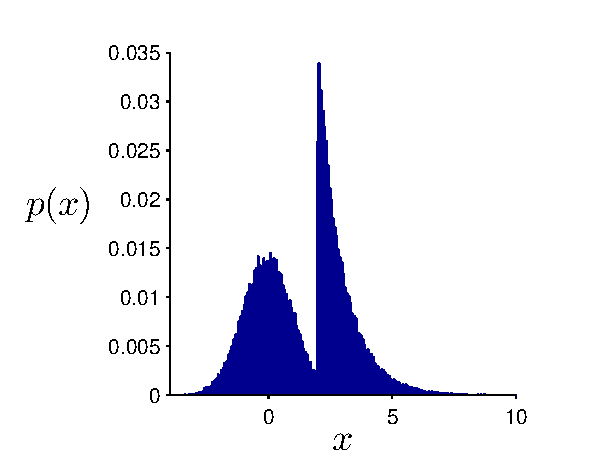
\includegraphics[width=0.45\textwidth]{figures/xmarg}
	  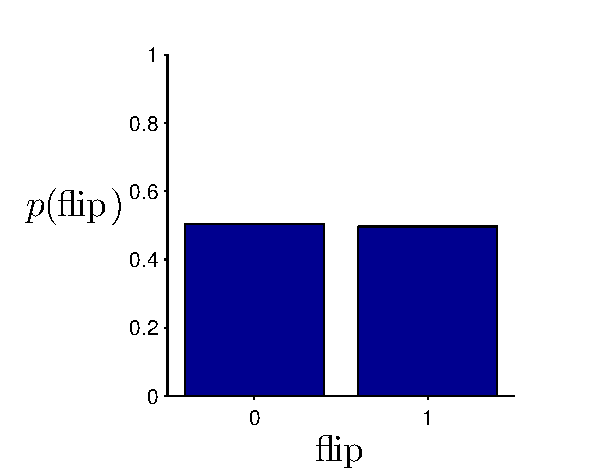
\includegraphics[width=0.45\textwidth]{figures/flipmarg}}
  \only<3>{
	  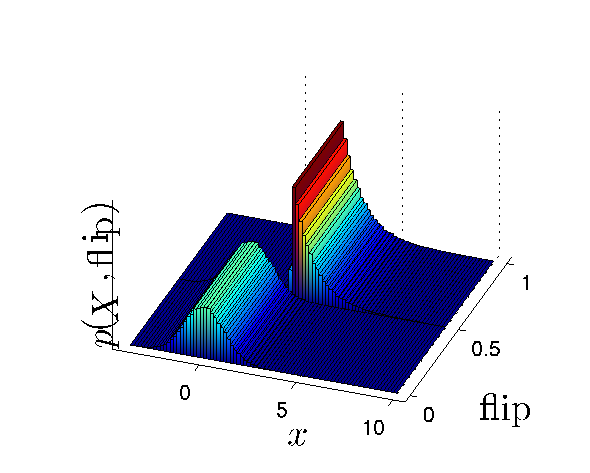
\includegraphics[width=0.45\textwidth]{figures/joint}
	  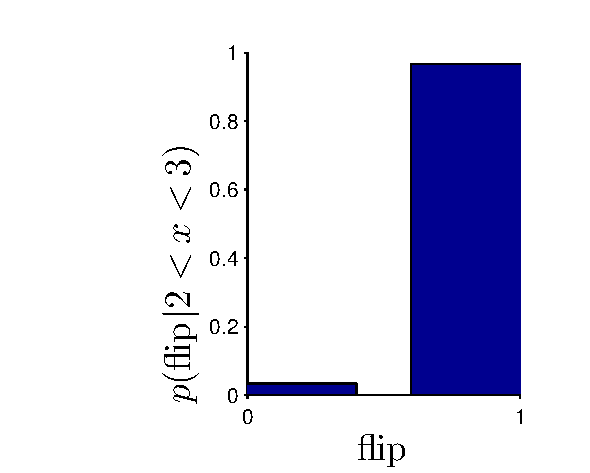
\includegraphics[width=0.45\textwidth]{figures/flipcond}}	  
%	  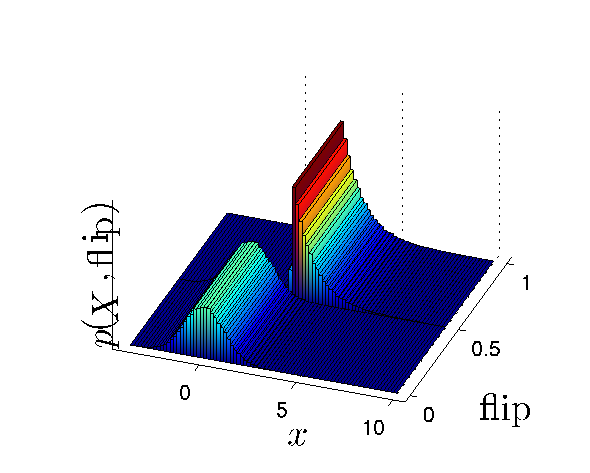
\includegraphics[width=0.4\textwidth]{figures/joint}
	 % \end{figure}
  \end{block}
\end{frame}

\begin{frame}{Probabilistic Programs vs Probabilistic Programming}
\TBD{DD}
\TBD{Move this between earlier slides if sensible}
  \begin{block}{Once we've defined a prior, what do we want to do with it?}  
  The PP defines $P(D,N,H)$, we choose D to be the subset of variables we observe, H the set of variables we're interested in, and N the set of variables that we're not interested in, so we'll integrate them out.  We want to get to $P(H|D)$
  \end{block}
      \begin{block}{Probabilistic Programming}
      \begin{enumerate}
        \item Usually refers to doing inference when a PP specifies your prior.
        \item 
      \end{enumerate}
    \end{block}
    TODO: Show the two possibilities of conditioning in th eprevious program
\end{frame}

\begin{frame}{Can we develop generic inference for all PPs?}
  \begin{block}{Rejection sampling}
    \begin{enumerate}
      \item Run the program with a fresh source of random numbers
      \item If condition $D$ is true, record $H$ as a sample, else ignore the sample
      \item Repetere infinitum
    \end{enumerate}
  \end{block}
  \begin{block}{Example}
    %\vspace{0.5\baselineskip}
    %\centering
    %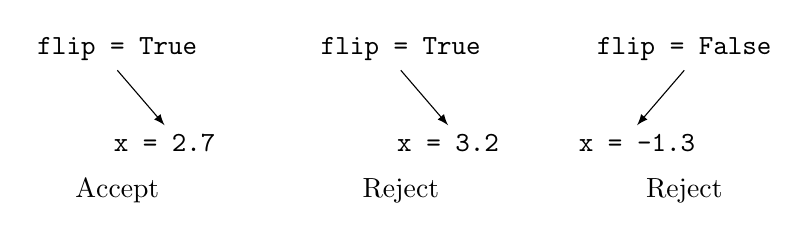
\begin{tikzpicture}[->,>=stealth',scale=1.2] 
  \begin{scope}[xshift=-3cm]
    \node[mybox] (root) at (0,0) {\texttt{flip = True}};
    \node[mybox] (left) at (-0.5,-1) {};
    \node[mybox] (right) at (0.5,-1) {\texttt{x = 2.7}};
    %\draw[-latex] (root.south) -- (left.north);
    \draw[-latex] (root.south) -- (right.north);
    \node[mybox] at (0,-1.5) {Accept};
  \end{scope}
  \begin{scope}[xshift=-0cm]
    \node[mybox] (root) at (0,0) {\texttt{flip = True}};
    \node[mybox] (left) at (-0.5,-1) {};
    \node[mybox] (right) at (0.5,-1) {\texttt{x = 3.2}};
    %\draw[-latex] (root.south) -- (left.north);
    \draw[-latex] (root.south) -- (right.north);
    \node[mybox] at (0,-1.5) {Reject};
  \end{scope}
  \begin{scope}[xshift=+3cm]
    \node[mybox] (root) at (0,0) {\texttt{flip = False}};
    \node[mybox] (left) at (-0.5,-1) {\texttt{x = -1.3}};
    \node[mybox] (right) at (0.5,-1) {};
    \draw[-latex] (root.south) -- (left.north);
    %\draw[-latex] (root.south) -- (right.north);
    \node[mybox] at (0,-1.5) {Reject};
  \end{scope}
\end{tikzpicture}

    \begin{columns}
      \begin{column}{.4\textwidth}
        \begin{alltt}
flip = rand < 0.5
if flip
\ \ x = randg + 2
else
\ \ x = randn
end
\end{alltt}

      \end{column}
      \begin{column}{.4\textwidth}
        
        \only<1>{
        \begin{alltt}
	        \
	        
	        \ 
	        
	        \ 
	        
	        \
	        
	        \
	        
	        \

        \end{alltt}
        }
        \only<2>{
        \begin{alltt}
	        >>True
	        
	        \ 
	        
	        \ 
	        
	        \
	        
	        \
	        
	        \

        \end{alltt}
        }
        \only<3>{
        \begin{alltt}
	        >>True
	        
	        \ 
	        
	        >>2.7
	        
	        \
	        
	        \
	        
	        \

        \end{alltt}
        }
        \only<4>{
        \begin{alltt}
	        \
	        
	        \ 
	        
	        \ 
	        
	        \
	        
	        \
	        
	        \

        \end{alltt}
        }
        \only<5>{
        \begin{alltt}
	        >>True
	        
	        \ 
	        
	        \ 
	        
	        \
	        
	        \
	        
	        \

        \end{alltt}
        }
        \only<6>{
        \begin{alltt}
	        >>True
	        
	        \ 
	        
	        >>3.2
	        
	        \
	        
	        \
	        
	        \

        \end{alltt}
        }
        \only<7>{
        \begin{alltt}
	        \
	        
	        \ 
	        
	        \ 
	        
	        \
	        
	        \
	        
	        \

        \end{alltt}
        }
        \only<8>{
        \begin{alltt}
	        >>True
	        
	        \ 
	        
	        \ 
	        
	        \
	        
	        \
	        
	        \

        \end{alltt}
        }
        \only<9>{
        \begin{alltt}
	        >>True
	        
	        \ 
	        
	        >>2.1
	        
	        \
	        
	        \
	        
	        \

        \end{alltt}
        }
        \only<10>{
        \begin{alltt}
	        \
	        
	        \ 
	        
	        \ 
	        
	        \
	        
	        \
	        
	        \

        \end{alltt}
        }
        \only<11>{
        \begin{alltt}
	        >>False
	        
	        \ 
	        
	        \ 
	        
	        \
	        
	        \
	        
	        \

        \end{alltt}
        }
        \only<12>{
        \begin{alltt}
	        >>False
	        
	        \ 
	        
	        \
	        
	        \
	        
	        >>-1.3
	        
	        \

        \end{alltt}
        }
        \only<13>{
        \begin{alltt}
	        \
	        
	        \ 
	        
	        \ 
	        
	        \
	        
	        \
	        
	        \

        \end{alltt}
        }
        \only<14>{
        \begin{alltt}
	        >>False
	        
	        \ 
	        
	        \ 
	        
	        \
	        
	        \
	        
	        \

        \end{alltt}
        }
        \only<15>{
        \begin{alltt}
	        >>False
	        
	        \ 
	        
	        \
	        
	        \
	        
	        >>2.3
	        
	        \

        \end{alltt}
        }

      \end{column}
    \end{columns}
  \end{block}
  \begin{block}{This produces samples over the \emph{execution trace}}
    \eg 
    \onslide<3->{\texttt{(True, 2.7)},}
    \onslide<9->{\texttt{(True, 2.1)},}
    \onslide<15->{\texttt{(False, 2.3)}, \dots}
  \end{block}
\end{frame}

\begin{frame}{Can we be more efficient?}
  \begin{block}{MCMC}
    \begin{enumerate}
  \onslide<1->{
    \item Start with a trace
    \begin{itemize}
      \item \texttt{(True, 2.3)}
    \end{itemize}
  }
  \onslide<2->{
    \item Change one random decision, discarding subsequent decisions
    \begin{itemize}
      \item \texttt{(False,)}
    \end{itemize}
  }
  \onslide<3->{
    \item Sample subsequent decisions
    \begin{itemize}
      \item \texttt{(False, -0.9)}
    \end{itemize}
  }
  \onslide<4->{
    \item Accept with appropriate (RJ)MCMC acceptance probability
    \begin{itemize}
      \item Reject, does not satisfy observation (\ie likelihood is zero)
    \end{itemize}
  }
\end{enumerate}

  \end{block}
\end{frame}

\begin{frame}{Can we be more efficient?}
  \begin{block}{MCMC}
    \begin{enumerate}
  \onslide<1->{
    \item Start with a trace
    \begin{itemize}
      \item \texttt{(True, 2.3)}
    \end{itemize}
  }
  \onslide<2->{
    \item Change one random decision, discarding subsequent decisions
    \begin{itemize}
      \item \texttt{(True, 2.9)}
    \end{itemize}
  }
  \onslide<3->{
    \item Sample subsequent decisions
    \begin{itemize}
      \item Nothing to do
    \end{itemize}
  }
  \onslide<4->{
    \item Accept with appropriate (RJ)MCMC acceptance probability
    \begin{itemize}
      \item Accept, maybe
    \end{itemize}
  }
\end{enumerate}

  \end{block}
\end{frame}

\begin{frame}{PP via MCMC - notation}
  \TBD{Maybe include parameter of random bitstring for notational consistency}
  \begin{block}{}
    Following Wingate et alia we represent the unconditioned PP as a parameterless function $f$
    \newline
    
    Evaluating $f$ results in random choices which are denoted as
    \begin{equation*}
      x_k = f_{k|x_1,\ldots,x_{k-1}} \sim p_{t_k}(.|\theta_{k},x_1,\ldots,x_{k-1}).
    \end{equation*}
    
    The density / probability of a particular evaluation is then
    \begin{equation*}
      p(x) = \prod_{k=1}^K p_{t_k}(x_k|\theta_{k},x_1,\ldots,x_{k-1}).
    \end{equation*}
    
    We then perform MCMC over the $x_k$ \ie the execution trace.
    
  \end{block}
\end{frame}

\begin{frame}{MCMC over execution traces}
  \begin{enumerate}
    \item Select a random $x_k = f_k$ in the execution trace
    \item Propose a new value $x_k' \sim K_{t_k}(.|x_k,\theta_k)$
    \item Run the program to determine all subsequent choices $(x_l' : l > k)$, reusing current choices where possible
    \item Propose moving from the state $(x_1,\ldots,x_K)$ to $(x_1,\ldots,x_{k-1},x_k',\ldots,x_{K'}')$
    \item Accept the change with the appropriate reversible jump MCMC acceptance probability
    %\begin{itemize}
      %\item $K_{t_k}(x_k'|x_k,\theta_k),\,K_{t_k}(x_k|x_k',\theta_k),\,p_{t_k}(x_k|\theta_{k},x_1,\ldots,x_{k-1})$
      %\item $\prod_{i=k}^K p_{t_i}(x_i|\theta_{i},x_1,\ldots,x_{i-1}),\,\prod_{i=k}^{K'} p_{t_i'}(x_i'|\theta_{i}',x_1,\ldots,x_{k-1},x_k',\ldots,x_{i-1}')$
      %\item \ie $\frac{K_{t_k}(x_k|x_k',\theta_k)\prod_{i=k}^{K'} p_{t_i'}(x_i'|\theta_{i}',x_1,\ldots,x_{k-1},x_k',\ldots,x_{i-1}')}{K_{t_k}(x_k'|x_k,\theta_k)\prod_{i=k}^K p_{t_i}(x_i|\theta_{i},x_1,\ldots,x_{i-1})}$
    %\end{itemize}
  \end{enumerate}
  \begin{equation*}
    \frac{K_{t_k}(x_k|x_k',\theta_k)\prod_{i=k}^{K'} p_{t_i'}(x_i'|\theta_{i}',x_1,\ldots,x_{k-1},x_k',\ldots,x_{i-1}')}{K_{t_k}(x_k'|x_k,\theta_k)\prod_{i=k}^K p_{t_i}(x_i|\theta_{i},x_1,\ldots,x_{i-1})}
  \end{equation*}
\end{frame}

%\begin{frame}{Worked example}
%\TBD{If there is time}
%\end{frame}

\begin{frame}{Further generic inference methods}
\TBD{Dave}
Now that we have separated inference and model design, what inference methods could we do

\eg HMC, parallel tempering, etc. (with citations)

Remember graphical models (fancy algorithms that work in certain model classes)
\end{frame}

\begin{frame}{Main strength}
\TBD{Dave}
Writing non-parametric models easy

Only need to evaluate samples from non-parametric objext lazily
\end{frame}

\begin{frame}{Nonparametric example}
If we can sample from the prior of a nonparametric model using finite resources (with probability 1), then we can apply probabilistic programming.
\newline

We can do this simply for a number of NPB models. In particular, we might be interested in models that use Dirichlet processes. We give an example in MATLAB
\newline

Point is that even if one can sample from posterior finitely, still might not be able to do PP. (PP requires weaker(?) condition that we can sample from prior finitely). Active research to produce finite algorithms to sample from nonparametric objects \eg Dan
\end{frame}

\begin{frame}{Example: Mixture of Gaussians}
  \begin{columns}
    \begin{column}{.5\textwidth}
      \begin{block}{Generative model}
        \begin{eqnarray*}
          (\mu_i)_{i=1\ldots k} & \simiid & \mathcal{N}(0, 1) \\
          (\pi_i)_{i=1\ldots k} & \sim & \textrm{Dir}(\alpha) \\
          \Theta & := & \sum_{i=1}^k \pi_i \delta_{\mu_i} \\
          (\theta_i)_{i=1\ldots n} & \simiid & \Theta \\
          (x_i)_{i=1\ldots n} & \simiid & \mathcal{N}(\theta_i, 1)
        \end{eqnarray*}
      \end{block}
    \end{column}
    \begin{column}{.5\textwidth}
      \begin{block}{(Pseudo) MATLAB code}
        \vspace{0.75\baselineskip}
        \begin{alltt}
          mu = randn(k,1);

          pi = dirichlet(k, alpha);


          for i = 1:n
            
          \ \ theta = mu(mnrnd(1,pi));
          
          \ \ x(i) \ = theta + randn;
            
          end
        \end{alltt}
        \vspace{0.75\baselineskip}
      \end{block}
    \end{column}
  \end{columns}
\end{frame}

\begin{frame}{Stolen stick breaking slide}
????
\end{frame}

\begin{frame}{Example: Infinite mixture of Gaussians}
  \begin{block}{Change to generative model}
    \begin{equation*}
      \Theta := \sum_{i=1}^k \pi_i \delta_{\mu_i} \to \Theta \sim \textrm{DP}(\alpha, \mathcal{N}(0,1))
    \end{equation*}
  \end{block}
  \begin{block}{(Pseudo) MATLAB code - stick breaking construction}
    \begin{alltt}
      sticks = []; atoms = [];
      
      for i = 1:n
      
      \ \ p = rand;
      
      \ \ while p > sum(sticks)
      
      \ \ \ \ sticks(end+1) = (1-sum(sticks)) * betarnd(1, alpha);
      
      \ \ \ \ atoms(end+1) \ = randn;
      
      \ \ end
      
      \ \ theta(i) = atoms(find(cumsum(sticks)>=p, 1, 'first'));
      
      end

      x = theta' + randn(n, 1);
    \end{alltt}
  \end{block}
\end{frame}

\begin{frame}{Stochastic memoisation}
Mention that stochastic memoisation is just stick/breaking or urn scheme and they make a fuss because it is lazy evaluation / functional calls which are ok due to exhangeability.
\end{frame}

\begin{frame}{PP timeline / videos / whatever}

Infer.net?
\end{frame}

\end{document}


